% !TEX root = main.tex
\section{SAT Solving Algorithms}
\begin{mytitle}[The SAT problem] Given a propositional formula with free variables, can we find a way to assign the free variables to make the formula true?
\end{mytitle}
\begin{mytitle}[SAT solver] An efficient tool to automatically answer this question. This is the classic NP-complete problem. Thus the worst case complexity is exponential. But average cases encountered in practice can be handled much faster.
\end{mytitle}
\subsection{Definitions}
\begin{mytitle}[Propositional variables] An alphabet $p, q, r, \ldots, p_1, p_2$
\end{mytitle}
\begin{mytitle}[Propositional formulas] $A, B ::= p\ |\ \top\ |\ \bot\ |\ \lnot A\ |\ A \land B\ |\ A \lor B\ |\ A \To B\ |\ A \Leftrightarrow B$
\end{mytitle}
\begin{mytitle}[Propositional model] A propositional model $M$ maps propositional values to truth values
\end{mytitle}
\begin{mytitle}[Satisfaction] A formula $A$ is satisfied by a model $M$, written $M \models A$, by usual semantics.
\end{mytitle}
\begin{mytitle}[Validity] A formula $A$ is valid iff for all models $M$ holds $M \models A$.
\end{mytitle}
\begin{mytitle}[Satisfiability] A formula $A$ is satisfiable iff for some model $M$ holds $M \models A$.
\end{mytitle}
\begin{mytitle}[Unsatisfiability] A formula $A$ is unsatisfiable iff for no model $M$ holds $M \models A$.
\end{mytitle}
\begin{mytitle}[Entailment] A formula $A$ entails a formula $B$, written $A \models B$, iff for all models $M$ holds that if $M \models A$ then $M \models B$.
\end{mytitle}
\begin{mytitle}[Equivalence] Formulas $A$ and $B$ are equivalent, written $A \equiv B$, iff for all models $M$ holds $M \models A$ iff $M \models B$.
\end{mytitle}
\begin{mytitle}[Propositional Equivalences]\hfill
\begin{itemize}
    \item $\lnot\lnot A \equiv A$ and $\lnot\top\equiv\bot$ and $\lnot A \equiv A \To \bot$
    \item $A \land B \equiv B \land A$ and $A \lor B \equiv B \lor A$ and $A \Leftrightarrow B \equiv B \Leftrightarrow A$
    \item $A\land \top \equiv A$ and $A\land \bot \equiv \bot$ and $A\lor \top \equiv \top$ and $A\lor \bot \equiv A$
    \item $(A\land B) \lor C \equiv (A\lor C) \land (B\lor C)$ and $(A\lor B) \land C \equiv (A\land C) \lor (B \land C)$
    \item $\lnot(A\lor B) \equiv \lnot A \land \lnot B$ and $\lnot(A\land B) \equiv \lnot A \lor \lnot B$
    \item $A\Leftrightarrow B \equiv (A\To B) \land (B\To A) \equiv (A\land B) \lor (\lnot A \land \lnot B)$
    \item $A\To B\lor C \equiv A\land \lnot B \To C$ and $A\land B \To C \equiv A \To \lnot B \lor C$
\end{itemize}
\end{mytitle}
\begin{mytitle}[Literal] A literal is a variable or the negation of one. We write $\sim l$ for the negation of literal $l$.
\end{mytitle}
\begin{mytitle}[Clause] A clause is a disjunction of literals $p\lor q\lor r\lor \ldots$. The empty clause is defined to be $\bot$.
\begin{mytitle}[Unit Clause] A unit clause is a single literal.
\end{mytitle}
\begin{mytitle}[Conjunctive Normal Form CNF] A formula is in conjunctive normal form iff it is a conjunction of clauses. An empty conjunction is defined to be $\top$.
\end{mytitle}
\end{mytitle}

\subsection{DPLL Algorithm}
\begin{mytitle}[Equi-Satisfiability] $A$ and $B$ are equi-satisfiable iff either both or neither are satisfiable.
\end{mytitle}
\begin{mytitle}[How SAT solving algorithms operate] SAT solving algorithms typically rewrite the input formula into an equi-satisfiable one in CNF, then rewrite the formula into further equi-satisfiable CNF formulas and/or perform a back-tracking search to explore different potential models. They terminate when the current formula is clearly equivalent to true or false. 
\end{mytitle}
\begin{mytitle}[Simple Conversion to CNF]\hfill
\begin{enumerate}
    \item Rewrite all $A\To B$ and $A \Leftrightarrow B$.
    \item Push all negations inward.
    \item Rewrite $\lnot\lnot A$ to $A$.
    \item Eliminate $\top$ and $\bot$.
    \item Distribute disjunctions over conjunctions.
    \item Simplify.
\end{enumerate}
\end{mytitle}
\begin{mytitle}[Davis-Putnam-Logemann-Loveland DPLL Algorithm] We assume an input formula $A$ in CNF, equivalently representable as a set of clauses or a set of literals. E.g. $(p\lor r) \land (\lnot r\lor s\lor t)$ becomes $\{\{p,r\}, \{\lnot r, s, t\}\}$. The algorithm rewrites clauses until the set is empty, indicating $sat$, or a clause is empty, indicating $unsat$. The algorithm builds up a partial model $M$, which assigns truth values to only some variables. We represent partial models using finite sets of literals. E.g. $M = \{p, \lnot r\}$.
    \begin{mysubtitle}[Pure Literal Rule] If $p$ occurs only positively/negatively in $A$, delete clauses of $A$ in which $p$ occurs. Then update $M$ to $M\cup \{p\} /M\cup \{\lnot p\}$.
    \end{mysubtitle}
    \begin{mysubtitle}[Unit Propagation] If $l$ is a unit clause in $A$, remove all clauses from $A$ which have $l$ as a disjunct and update all clauses in $A$ containing $\sim l$ by removing that disjunct. Then update $M$ to $M\cup\{l\}$.
    \end{mysubtitle}
    \begin{mysubtitle}[Decision] If $p$ occurs both positively and negatively in clauses of $A$, apply the algorithm to $(M\cup \{p\}, A\land p)$. If we get $(sat, M)$ then return that. Otherwise, apply the algorithm to $(M\cup \{\lnot p\}, A\land \lnot p)$ and return the result.
    \end{mysubtitle}
\end{mytitle}
\begin{mytitle}[Implication graph] We can visualize the search for a model with an implication graph. We use a red circle to indicate decision literals and red arrows to indicate the order of decisions. We use blue circles for literals added due to unit propagation and blue arrows to record its dependencies. When a clause becomes empty, we add a green conflict node and add blue arrows analogously to unit propagation, so we can see which decisions had to do with the conflict.
\end{mytitle}

\subsection{CDCL Algorithm}
\begin{mytitle}[Conflict-Driven Clause Learning CDCL Algorithm] This algorithm is better than DPLL in practice, but less so for random SAT examples. In practice, clauses are also periodically removed during SAT solver runs.
    \begin{mysubtitle}[Back-jumping] When a conflict is found, identify the relevant decision literals, then pop the relevant literal and as many other non-relevant literals from the stack as possible. Then flip the relevant literal and go on.
    \end{mysubtitle}
    \begin{mysubtitle}[Clause Learning] When a conflict is found, draw a cut in the graph, separating the conflict node from all decision literals. All edges should go from left to right. For nodes with outgoing edges crossing the boundary, save the disjunction of the negations of their literals. When back-jumping, conjoin this new clause to the current formula.
    \end{mysubtitle}
\end{mytitle}

\begin{center}
\begin{minipage}{0.49\textwidth}
\begin{center}
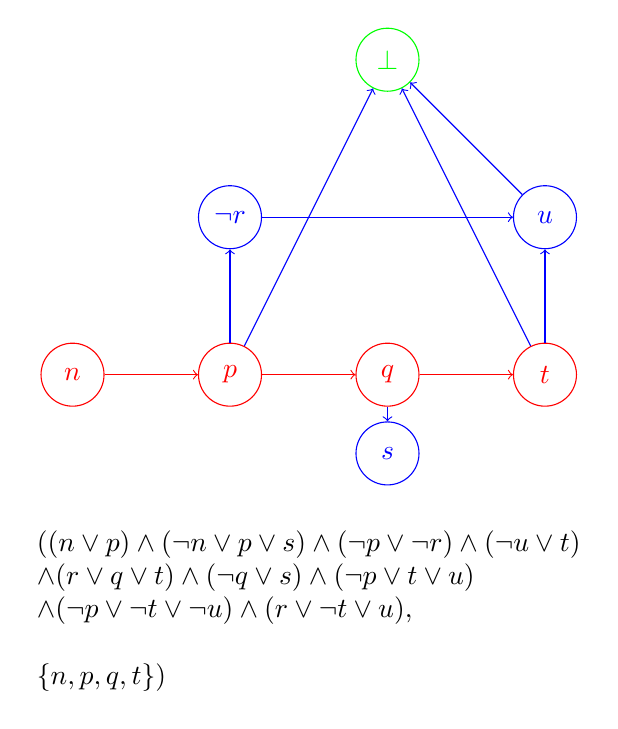
\begin{tikzpicture}
\node (n) [draw, circle, red, align=center, minimum size=0.8cm] at (0,0) {$n$};
\node (p) [draw, circle, red, align=center, minimum size=0.8cm] at (2,0) {$p$};
\node (q) [draw, circle, red, align=center, minimum size=0.8cm] at (4,0) {$q$};
\node (t) [draw, circle, red, align=center, minimum size=0.8cm] at (6,0) {$t$};
\node (s) [draw, circle, blue, align=center, minimum size=0.8cm] at (4,-1) {$s$};
\node (r) [draw, circle, blue, align=center, minimum size=0.8cm] at (2,2) {$\lnot r$};
\node (u) [draw, circle, blue, align=center, minimum size=0.8cm] at (6,2) {$u$};
\node (conflict) [draw, circle, green, align=center, minimum size=0.8cm] at (4,4) {$\bot$};

\draw [->, red] (n) -- (p);
\draw [->, red] (p) -- (q);
\draw [->, red] (q) -- (t);

\draw [->, blue] (p) -- (r);
\draw [->, blue] (p) -- (conflict);
\draw [->, blue] (q) -- (s);
\draw [->, blue] (t) -- (u);
\draw [->, blue] (t) -- (conflict);
\draw [->, blue] (r) -- (u);
\draw [->, blue] (u) -- (conflict);

\node (formula1) [align=left] at (3, -3) {($(n\lor p) \land(\lnot n\lor p\lor s) \land (\lnot p \lor \lnot r) \land (\lnot u \lor t)$ \\ $ \land (r\lor q \lor t) \land(\lnot q\lor s) \land (\lnot p\lor t \lor u)$ \\ $\land (\lnot p\lor \lnot t\lor \lnot u) \land (r\lor \lnot t\lor u)$, \\
\\
$\{n, p, q, t\}$)};
\end{tikzpicture}
\end{center}
\end{minipage}
\begin{minipage}{0.49\textwidth}
\begin{center}
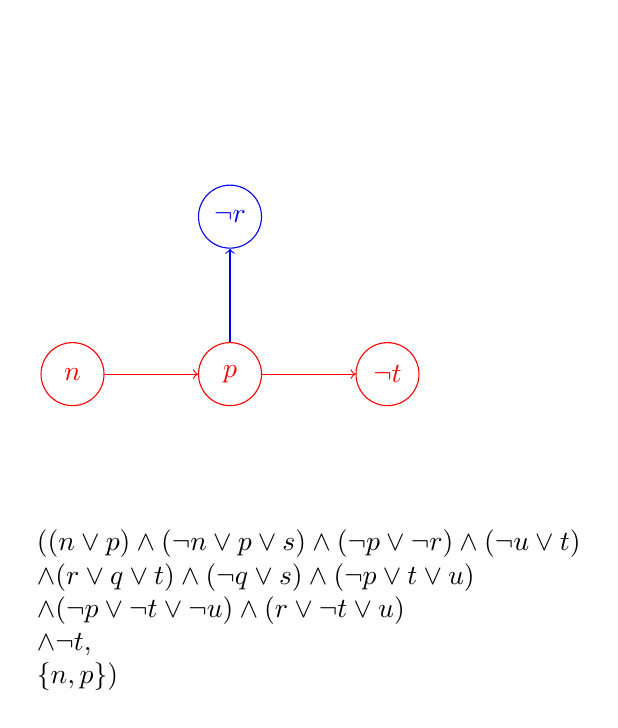
\begin{tikzpicture}
\node (n) [draw, circle, red, align=center, minimum size=0.8cm] at (0,0) {$n$};
\node (p) [draw, circle, red, align=center, minimum size=0.8cm] at (2,0) {$p$};
\node (t) [draw, circle, red, align=center, minimum size=0.8cm] at (4,0) {$\lnot t$};
\node (r) [draw, circle, blue, align=center, minimum size=0.8cm] at (2,2) {$\lnot r$};
\node (x) [minimum size=0.8cm] at (4,4) {};

\draw [->, red] (n) -- (p);
\draw [->, red] (p) -- (t);

\draw [->, blue] (p) -- (r);

\node (formula1) [align=left] at (3, -3) {($(n\lor p) \land(\lnot n\lor p\lor s) \land (\lnot p \lor \lnot r) \land (\lnot u \lor t)$ \\ $ \land (r\lor q \lor t) \land(\lnot q\lor s) \land (\lnot p\lor t \lor u)$ \\ $\land (\lnot p\lor \lnot t\lor \lnot u) \land (r\lor \lnot t\lor u)$ \\
$\boldsymbol{\land \lnot t}$, \\
$\{n, p\}$)};
\end{tikzpicture}
\end{center}
\end{minipage}
\captionof{figure}{Example implication graph before and after back-jumping.}
\end{center}

\begin{center}
\begin{minipage}{0.49\textwidth}
\begin{center}
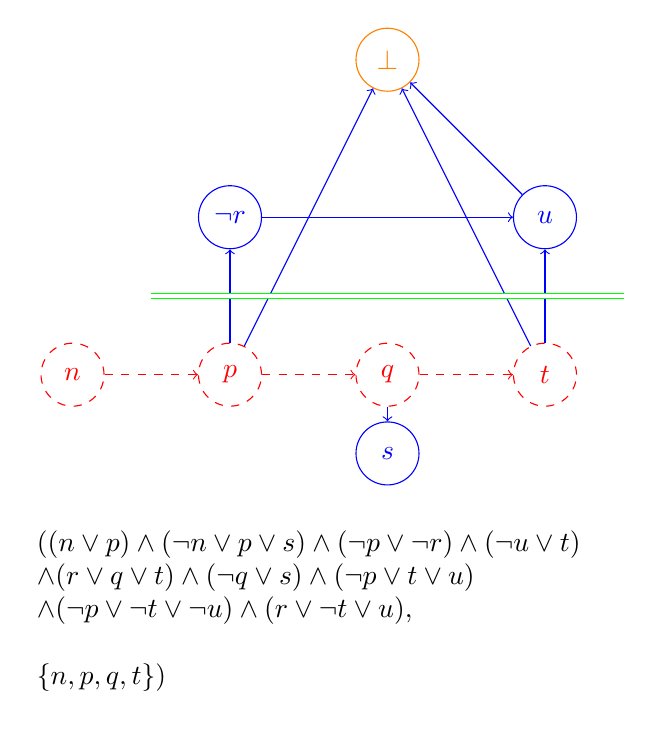
\begin{tikzpicture}
\node (n) [draw, dashed, circle, red, align=center, minimum size=0.8cm] at (0,0) {$n$};
\node (p) [draw, dashed, circle, red, align=center, minimum size=0.8cm] at (2,0) {$p$};
\node (q) [draw, dashed, circle, red, align=center, minimum size=0.8cm] at (4,0) {$q$};
\node (t) [draw, dashed, circle, red, align=center, minimum size=0.8cm] at (6,0) {$t$};
\node (s) [draw, circle, blue, align=center, minimum size=0.8cm] at (4,-1) {$s$};
\node (r) [draw, circle, blue, align=center, minimum size=0.8cm] at (2,2) {$\lnot r$};
\node (u) [draw, circle, blue, align=center, minimum size=0.8cm] at (6,2) {$u$};
\node (conflict) [draw, circle, orange, align=center, minimum size=0.8cm] at (4,4) {$\bot$};

\draw [->, dashed, red] (n) -- (p);
\draw [->, dashed, red] (p) -- (q);
\draw [->, dashed, red] (q) -- (t);

\draw [->, blue] (p) -- (r);
\draw [->, blue] (p) -- (conflict);
\draw [->, blue] (q) -- (s);
\draw [->, blue] (t) -- (u);
\draw [->, blue] (t) -- (conflict);
\draw [->, blue] (r) -- (u);
\draw [->, blue] (u) -- (conflict);

\draw [double, green, double distance=1.5] (1,1) -- (7,1);

\node (formula1) [align=left] at (3, -3) {($(n\lor p) \land(\lnot n\lor p\lor s) \land (\lnot p \lor \lnot r) \land (\lnot u \lor t)$ \\ $ \land (r\lor q \lor t) \land(\lnot q\lor s) \land (\lnot p\lor t \lor u)$ \\ $\land (\lnot p\lor \lnot t\lor \lnot u) \land (r\lor \lnot t\lor u)$, \\
\\
$\{n, p, q, t\}$)};
\end{tikzpicture}
\end{center}
\end{minipage}
\begin{minipage}{0.49\textwidth}
\begin{center}
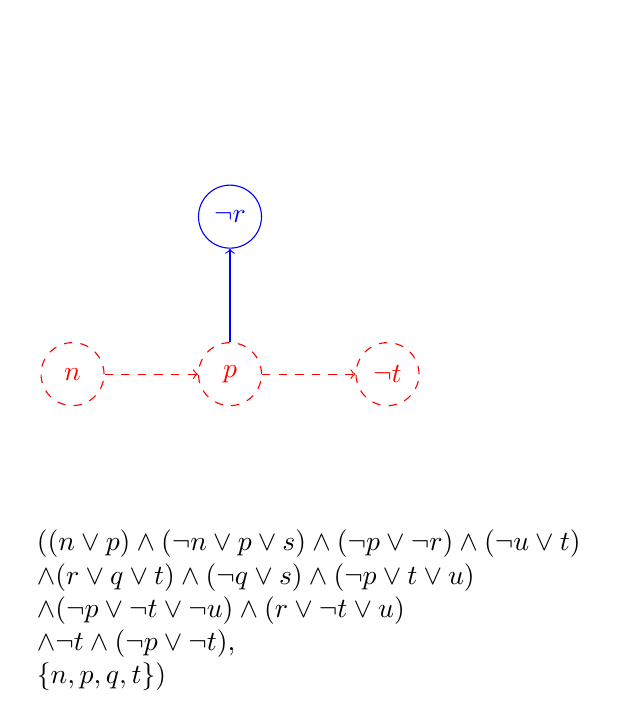
\begin{tikzpicture}
\node (n) [draw, dashed, circle, red, align=center, minimum size=0.8cm] at (0,0) {$n$};
\node (p) [draw, dashed, circle, red, align=center, minimum size=0.8cm] at (2,0) {$p$};
\node (t) [draw, dashed, circle, red, align=center, minimum size=0.8cm] at (4,0) {$\lnot t$};
\node (r) [draw, circle, blue, align=center, minimum size=0.8cm] at (2,2) {$\lnot r$};
\node (x) [minimum size=0.8cm] at (4,4) {};

\draw [->, dashed, red] (n) -- (p);
\draw [->, dashed, red] (p) -- (t);

\draw [->, blue] (p) -- (r);

\node (formula1) [align=left] at (3, -3) {($(n\lor p) \land(\lnot n\lor p\lor s) \land (\lnot p \lor \lnot r) \land (\lnot u \lor t)$ \\ $ \land (r\lor q \lor t) \land(\lnot q\lor s) \land (\lnot p\lor t \lor u)$ \\ $\land (\lnot p\lor \lnot t\lor \lnot u) \land (r\lor \lnot t\lor u)$\\
$\boldsymbol{\land \lnot t \land (\lnot p \lor \lnot t)}$, \\
$\{n, p, q, t\}$)};
\end{tikzpicture}
\end{center}
\end{minipage}
\captionof{figure}{Example implication graph before and after clause learning.}
\end{center}



